% ****** Start of file aipsamp.tex ******
%
%   This file is part of the AIP files in the AIP distribution for REVTeX 4.
%   Version 4.1 of REVTeX, October 2009
%
%   Copyright (c) 2009 American Institute of Physics.
%
%   See the AIP README file for restrictions and more information.
%
% TeX'ing this file requires that you have AMS-LaTeX 2.0 installed
% as well as the rest of the prerequisites for REVTeX 4.1
% 
% It also requires running BibTeX. The commands are as follows:
%
%  1)  latex  aipsamp
%  2)  bibtex aipsamp
%  3)  latex  aipsamp
%  4)  latex  aipsamp
%
% Use this file as a source of example code for your aip document.
% Use the file aiptemplate.tex as a template for your document.
\documentclass[%
 aip,
% jmp,
% bmf,
% sd,
% rsi,
 amsmath,amssymb,
%preprint,%
 reprint, floatfix%
%author-year,%
%author-numerical,%
% Conference Proceedings
]{revtex4-1}

\usepackage{graphicx}% Include figure files
\usepackage{dcolumn}% Align table columns on decimal point
\usepackage{bm}% bold math
%\usepackage[mathlines]{lineno}% Enable numbering of text and display math
%\linenumbers\relax % Commence numbering lines

\usepackage[utf8]{inputenc}
\usepackage[T1]{fontenc}
\usepackage{mathptmx}
\usepackage{mathtools}
\usepackage{etoolbox}
\usepackage{booktabs}
\usepackage{multirow}
\usepackage{subcaption}
\usepackage{gensymb}
\usepackage{siunitx}
\usepackage[version=4]{mhchem}
\usepackage{bm}
\DeclareSIUnit\gauss{G}
\DeclareSIUnit{\angstrom}{\textup{\AA}}
\usepackage[hidelinks]{hyperref}
\hypersetup{
    colorlinks=true,
    linkcolor=blue,
    filecolor=magenta,      
    urlcolor=cyan,
    pdftitle={Overleaf Example},
    pdfpagemode=FullScreen,
    }

%% Apr 2021: AIP requests that the corresponding 
%% email to be moved after the affiliations
\makeatletter
\def\@email#1#2{%
 \endgroup
 \patchcmd{\titleblock@produce}
  {\frontmatter@RRAPformat}
  {\frontmatter@RRAPformat{\produce@RRAP{*#1\href{mailto:#2}{#2}}}\frontmatter@RRAPformat}
  {}{}
}%
\makeatother
\begin{document}

\preprint{AIP/123-QED}

\title[Study of lattice dynamics using LC oscillator circuits]{Study of lattice dynamics using LC oscillator circuits}
% Force line breaks with \\
\author{Maitrey Sharma}
 \affiliation{School of Physical Sciences, National Institute of Science Education and Research, HBNI, Jatni-752050, India.}%Lines break automatically or can be forced with \\
 \email{maitrey.sharma@niser.ac.in}

\date{\today}% It is always \today, today,
             %  but any date may be explicitly specified

\begin{abstract}
This experiment primarily deals with the study of the dynamics of lattice vibrations. Although a very complex many-body system which is difficult to solve both classically and quantum mechanically, we make approximation to simplify our system by considering nearby-only phenomena and harmonic potentials. We draw analogies with electrical domain using the admittance analogy and model our system mechanical system using circuit elements to study it electrically. We explore both simple Bravais lattice systems (same kind of atoms in a linear chain) and Bravais lattice with a basis systems (dissimilar atoms in the linear chain) and analyse them extensively. We also discuss the nature of phonons and their properties and how they can play vital role in field of condensed matter physics.
\end{abstract}

\maketitle 


\begin{quotation}
\textit{If you want to find the secrets of the universe, think in terms of energy, frequency and vibration.}
\newline
\hspace*{0pt}\hfill Nikola Tesla
\end{quotation}

\section{Introduction}
    Almost all solids with the exception of amorphous solids and glasses have periodic arrays of atoms which form a crystal lattice. When a mechanical wave travels through a fluid, its (fluid's) constituent molecules begin to vibrate about their respective equilibrium positions. Moreover, since a wave transports energy, propagation of wave essentially means propagation of phase. A similar situation is observed in solids. When mechanical, thermal or electrical energy is supplied to a solid, its constituent atoms are set into vibration about their respective equilibrium sites resulting into wave propagation.
    \par
    In this experiment, we will study wave propagation through monoatomic and diatomic crystals made of discrete atoms. As such, these are 3-D systems. However, it is instructive to first consider vibrations of particles arranged in a straight line. A 1-D system exhibits all essential features of a 3-D system. A dispersion relation is a relation which relates the wavelength or wavenumber of a wave to its frequency. If we can analyse this dispersion relation and characteristics of a linear chain of identical atoms it is possible to identify the different modes of vibration (in a simple Bravais lattice or a Bravais lattice with a basis, that is, a chain of two different types of atoms). The dispersion relation of the diatomic lattice exhibits some unique features, in addition to those exhibited by the dispersion curve of a monoatomic lattice. The vibrations of atoms in a crystal determine its thermal properties, X-ray scattering, neutron scattering etc.
    \begin{figure}
        \centering
        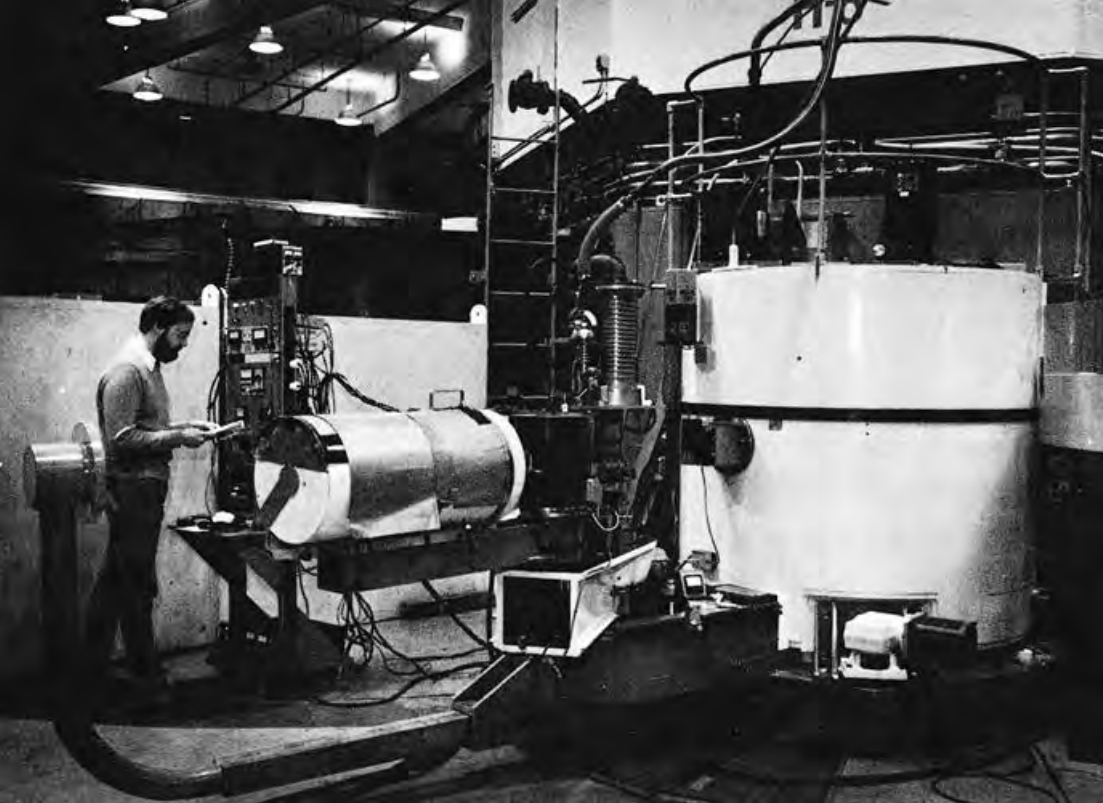
\includegraphics[scale = 0.37]{Figures/neutronscattering.png}
        \caption{A triple axis neutron spectrometer at Brookhaven. The dispersion curves of sodium for phonons propagating in the various directions can be determined by inelastic scattering of neutrons.}
        \label{fig:neutronscattering}
    \end{figure}
    \par
    We will see how the equations that govern the mechanics of the lattice are of the similar form of the equation which govern LC oscillations in a electrical circuit.
    \begin{figure}
        \centering
        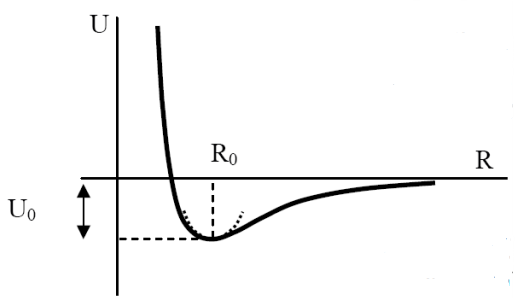
\includegraphics[scale = 0.75]{Figures/energy.png}
        \caption{Energy relationship with distance in a bound system}
        \label{fig:energy}
    \end{figure}
    \par
    Lattice vibrations can explain sound velocity, thermal properties, elastic properties and optical properties of materials. Lattice Vibration is the oscillations of atoms in a solid about the equilibrium position. For a crystal, the equilibrium positions form a regular lattice, due to the fact that the atoms are bound to neighboring atoms. The vibration of these neighboring atoms is not independent of each other. A regular lattice with harmonic forces between atoms and normal modes of vibrations are called lattice waves.

\section{Aim}
    We will be doing following experiments:
    \begin{enumerate}
        \item Study of the dispersion relation for the mono-atomic lattice-Comparison with theory.
        \item Determination of the cut-off frequency of the mono-atomic lattice.
        \item Study of the dispersion relation for the diatomic lattice — \textit{acoustical mode} and \textit{optical mode} energy gap and compare them with theory.
    \end{enumerate}
\section{Apparatus}
    The lattice dynamics kit has built-in audio oscillator that works on 220 V, 50 Hz and the only additional equipment needed is a general purpose cathode ray oscilloscope (CRO) having $XY$ mode. The Kit consists of the following parts:
    \begin{enumerate}
        \item Audio oscillator with amplitude control and facility to vary the frequency,
        \item Inductors and capacitors
        \item Connecting wires
        \item Breadboard,
        \item Oscilloscope
    \end{enumerate}


\section{Theory}
    We will begin our discussion by treating our system (1-D lattices) classically at first and wil later introduce the concept of \textit{phonons} in later sections. 
    \subsection{Lattice Dynamics of the Simple Bravais Lattice}
    A solid can be modelled as a 3-D coupled spring-mass system (figure (\ref{fig:ballsbyspring})). However, for simplicity, we consider a lattice shown in figure (\ref{fig:masschain}). Note that it consists of a large number of equally spaced, identical particles of mass $M$ held together by elastic springs, each of force constant $K$, in a linear array. These atoms can vibrate along the chain or at right angle to the chain. That is, the motion can be longitudinal or transverse. We first consider longitudinal motion. Let us choose $n$th atom as the origin.
    \begin{figure}
        \centering
        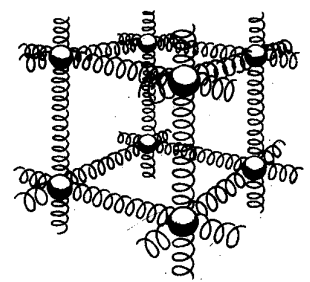
\includegraphics{Figures/ballsbyspring.png}
        \caption{A solid modelled as a system of balls connected by springs}
        \label{fig:ballsbyspring}
    \end{figure}
    \begin{figure}
        \centering
        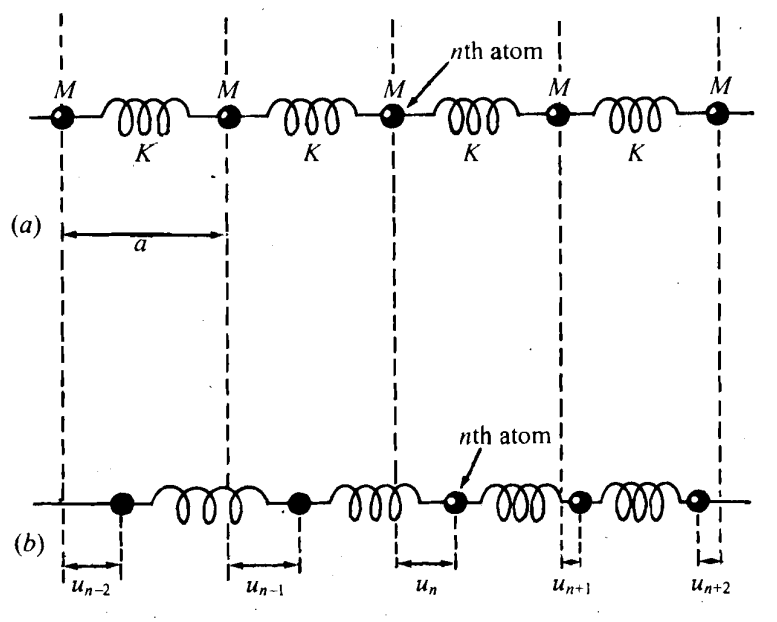
\includegraphics[scale = 0.5]{Figures/chainofmasses.png}
        \caption{A chain of masses $M$ connected by springs a) at equilibrium positions $x_n^0 = na$; and b) at displaced positions $x_n = na + u_n$}
        \label{fig:masschain}
    \end{figure}
    We assume that the last atom is joined to the first so as to form a closed loop. This enables us to visualize the linear chain as endless and thereby all atoms have identical environment. We denote the equilibrium spacing between the atoms by $a$. 
    \par
    If the $n$th atom is displaced from its equilibrium position, its equation of motion can be written as
    \begin{equation}
        M \dfrac{d^2 u_n}{dt^2} = -K (u_n - u_{n-1}) +K(u_{n+1}-u_n)
    \end{equation}
    or
    \begin{equation}
        M \dfrac{d^2 u_n}{dt^2} = K(u_{n+1}-2u_n+u_{n+1})
    \end{equation}
    where $u_n$, denotes the displacement of the $n$th atom from its equilibrium position. It is small compared to the interatomic distance. For solving this we take a solution in the form of a progressive wave: $u_n = A e^{-i(\omega t-kx_n^0)}$, where $A$ is the amplitude of the wave, $x_n^0(=na)$ denotes the equilibrium coordinate of the $n$th atom, $k$ is wave number and $\omega$ is angular frequency.
    \par
    Solving this leads to
    \begin{equation}
    \label{eq:dispersion}
        \omega = \omega_{0L} \Bigg| \sin \Bigg( \dfrac{ka}{2} \Bigg) \Bigg|
    \end{equation}
    where $\omega_{0L} = 2 \sqrt{\dfrac{K}{M}}$. Equation (\ref{eq:dispersion}) gives the dispersion relation for a linear array of same type of atoms.
    \par
    $\omega$ is independent of $n$, which means that all atoms would lead to the same algebraic relation between $\omega$ and $k$. Moreover, this relation is unique, i.e. corresponding to each $k$, there is a definite $\omega$. It means that the oscillations are uncoupled and correspond to normal modes. Further, the frequencies of all the normal modes lie in the range $-\pi/a < k < \pi/a$. This range of $k$ values defines the boundaries of the first \textit{Brillouin zone} for a 1-D crystal lattice.
    \begin{figure}
        \centering
        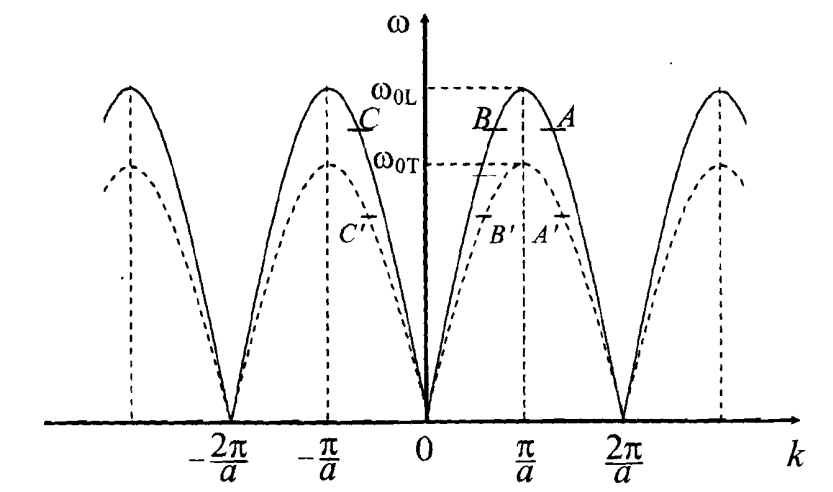
\includegraphics[scale = 0.49]{Figures/normalmodes.png}
        \caption{Normal mode frequencies for a linear chain of atoms}
        \label{fig:normalmode}
    \end{figure}
    \begin{figure}
        \centering
        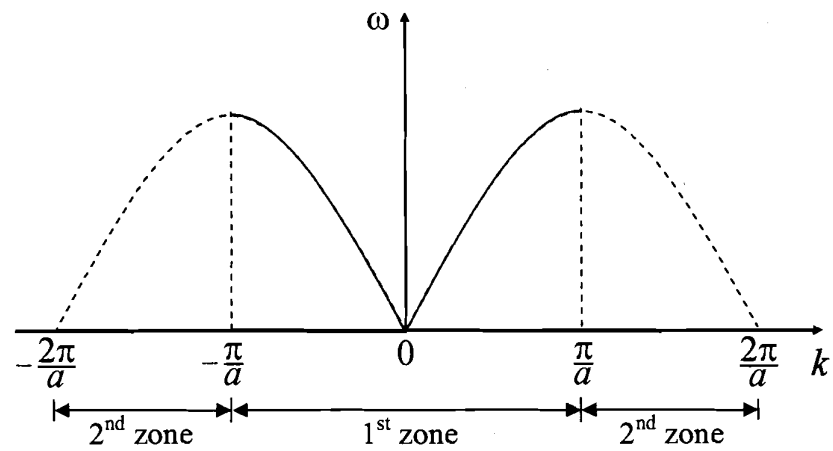
\includegraphics[scale = 0.45]{Figures/first2brillouin.png}
        \caption{First two Brillouin zones in the dispersion curve due to monatomic lattice}
        \label{fig:f2zones}
    \end{figure}
    \par
    \subsection{Lattice Dynamics of Bravais Lattice with a basis}
    A simple Bravais lattice can be generated by the translation of a unit cell - containing one particle. A Bravais lattice with a basis is generated by a simple translation when two different atoms are translated together.
    \par
    In the 1-D case, there are two possible ways to create a chain with a basis:
    \begin{itemize}
        \item The atoms are placed at equal distances but alternate atoms have different masses;
        \item All atoms are of equal mass but the distances between them are not uniform. 
    \end{itemize} 
    \begin{figure}
        \centering
        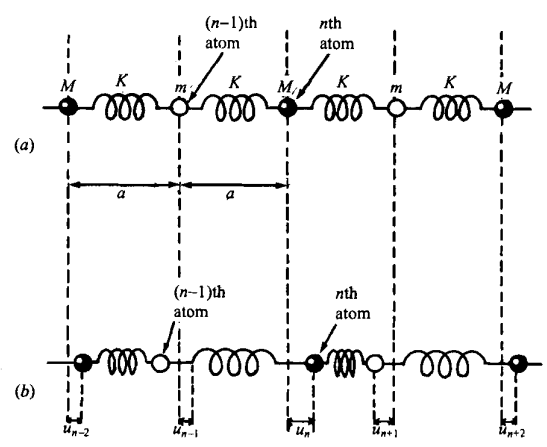
\includegraphics[scale = 0.5]{Figures/unequalchain.png}
        \caption{A chain of masses $M$ connected by springs a) at equilibrium positions $x_n^0 = na$; and b) at displaced positions $x_n = na + u_n$}
        \label{fig:uneqchain}
    \end{figure}
    Here we will consider the first case as it provides a model for ionic crystals. Let atomic masses with a basis be denoted by $M$ and $m$ ($m < M$) as shown in figure (\ref{fig:uneqchain}). As before, we suppose that the distance between the nearest neighbours is $a$. We can write down the equation of motion for longitudinal vibrations for the masses $M$ and $m$ as
    \begin{equation}
        M \dfrac{d^2 u_n}{dt^2} = K(u_{n+1}-2u_n+u_{n-1})
    \end{equation}
    and
    \begin{equation}
        m \dfrac{d^2 u_{n-1}}{dt^2} = K(u_{n}-2u_{n-1}+u_{n-2})
    \end{equation}
    Proceeding in the same manner as before, we assume the solutions of the form
    \begin{equation}
        u_n = A e^{-i(\omega t-kx_n^0)}
    \end{equation}
    for mass $M$ and
    \begin{equation}
        u_{n\pm1} = A \alpha e^{-i(\omega t- kx_{n \pm 1}^0)}
    \end{equation}
    for mass $m$.
    Solving this leads to
    \begin{equation}
    \label{eq:branch}
        \omega_{\pm}^2 = \dfrac{K(M+m)}{mM}\Bigg \{ 1 \pm \Big[ 1 - \dfrac{4mM}{(m+M)^2} \sin^2 ka \Big]^{1/2} \Bigg \}
    \end{equation}
    For a one to one correspondence between the state of vibration of the lattice and the wave vector $k$, the latter must be restricted to a range of values $\pi/a$. The range of the first Brillouin zone in this case is $-\pi/2a < k \leq \pi/2a$. Note that width of Brillouin zone for a lattice with a basis is half of that for a simple lattice.
    \begin{figure}
        \centering
        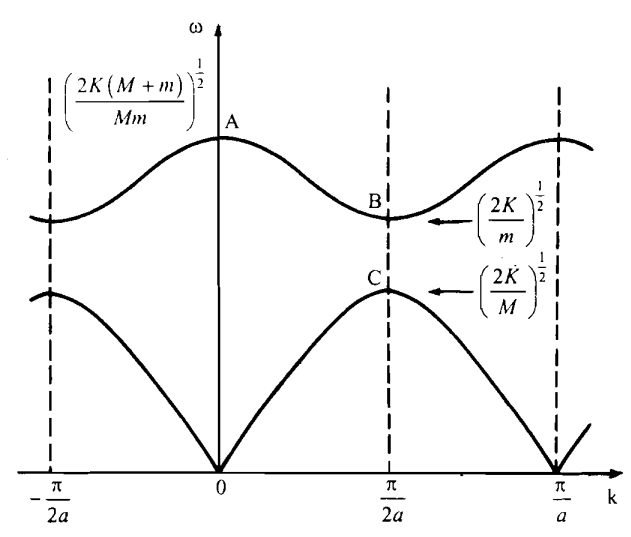
\includegraphics[scale = 0.55]{Figures/normalmodeuneq.png}
        \caption{Normal mode frequencies of a chain of two types of atom. At A the two types of atoms are oscillating in opposite phases with their centre of mass at rest; at B the lighter mass $m$ is oscillating and $M$ is at rest; and at C, $M$ is oscillating and $m$ is at rest}
        \label{fig:my_label}
    \end{figure}
    \par
    The branch which correspond to a non-zero value of $\omega$ for $k=0$ is called \textit{optical branch}. It is because the frequencies in this branch are of the order of infrared frequencies. The branch corresponding to $\omega=0$ for $k=0$ is called \textit{acoustical branch} because the corresponding frequencies are of the order of acoustical or supersonic vibrations.
    \par
    For small values of $k$, that is, for $k \rightarrow 0$, we have $\sin ka \approx ka$ and frequencies corresponding to optical and acoustical branches are obtained by simplifying equation (\ref{eq:branch}) as
    \begin{equation}
        \omega_o = \sqrt{\dfrac{2K(M+m)}{mM}} \Bigg( 1 - \dfrac{1}{2} \dfrac{mMk^2a^2}{(m+M)^2} \Bigg)
    \end{equation}
    and
    \begin{equation}
        \omega_a = \sqrt{\dfrac{2K}{M+m}} ka
    \end{equation}
    Note that in-between the optical branch and the acoustic branch, there is a band of frequencies which cannot propagate in a diatomic chain. However, it may also be noted that for $m=M$, this forbidden band disappears and we get $\omega$ versus $k$ curve similar to monoatomic chain (\ref{fig:normalmode}).
    \subsection{The Mobility Analogy}
    The mobility analogy, also called admittance analogy or Firestone analogy, is a method of representing a mechanical system by an analogous electrical system. By converting to an electrical representation, these tools in the electrical domain can be directly applied to a mechanical system without modification. The mathematical behaviour of the simulated electrical system is identical to the mathematical behaviour of the represented mechanical system. Each element in the electrical domain has a corresponding element in the mechanical domain with an analogous constitutive equation. The mobility analogy preserves the topology of the mechanical system, that is, elements that are in series in the mechanical system are in series in the electrical equivalent circuit and elements in parallel in the mechanical system remain in parallel in the electrical equivalent.
    \begin{figure}
        \centering
        \begin{subfigure}[b]{0.5\textwidth}
            \centering
            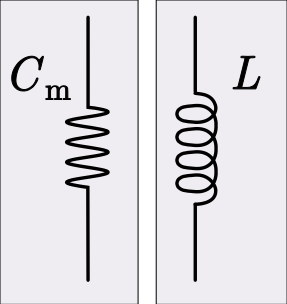
\includegraphics[scale = 0.35]{Figures/287px-Mobility_analogy_inductor.svg.png}
            \caption{The mechanical symbol for a compliance element (left) and its electrical analogy (right). The symbol is meant to be evocative of a spring.}
            \label{fig:ind}
        \end{subfigure}
        \hfill
        \begin{subfigure}[b]{0.5\textwidth}
            \centering
            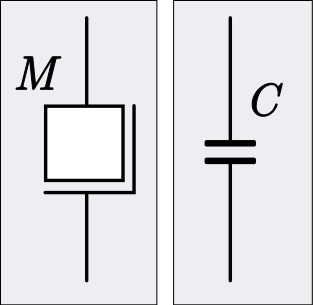
\includegraphics[scale = 0.35]{Figures/313px-Mobility_analogy_capacitor.svg.png}
            \caption{The mechanical symbol for a mass (left) and its electrical analogy (right). The square angle below the mass is meant to indicate that movement of the mass is relative to a frame of reference.}
            \label{fig:cap}
        \end{subfigure}
            \caption{The mobility analogy for inductor and capacitor}
            \label{fig:analogy}
    \end{figure}
    \par
    Consider inductance and capacitance. The mechanical analogy of inductance in the mobility analogy is compliance. It is more common in mechanics to discuss stiffness, the inverse of compliance. A mechanical component analogous to an inductor is a spring. An inductor is governed by the constitutive equation,
    \begin{equation}
        v = L \dfrac{di}{dt}
    \end{equation}
    The analogous equation in the mechanical domain is a form of Hooke's law,
    \begin{equation}
        u = C_m \dfrac{dF}{dt}
    \end{equation}
    where, $L$ is inductance, $t$ is time $C_m = 1/S$ is mechanical compliance and $S$ is stiffness.
    \par
    The mechanical analogy of capacitance in the mobility analogy is mass. A mechanical component analogous to a capacitor is a large, rigid weight. A capacitor is governed by the constitutive equation,
    \begin{equation}
        i = C \dfrac{dv}{dt}
    \end{equation}
    The analogous equation in the mechanical domain is Newton's second law of motion,
    \begin{equation}
        F = M \dfrac{du}{dt}
    \end{equation}
    \subsection{Everything Comes Together}
    Figure (\ref{fig:monolattice}) shows a mass and spring model for a one dimensional mono-atomic lattice. The particles having mass $m$ are connected by spring of force constant $f$.
    \begin{figure}
        \centering
        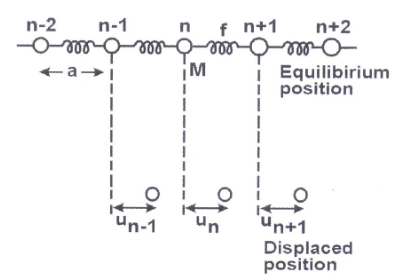
\includegraphics{Figures/monolattice.png}
        \caption{One-dimensional linear mono-atomic lattice; $a$ is the lattice constant; $f$ is the force constant; $M$ is the mass of the atom}
        \label{fig:monolattice}
    \end{figure}
    The equilibrium distance between the particles is $a$ and the array is assumed to be infinitely long. Assuming only the nearest neighbour interaction, the equation of the motion of the $n$th atom is given by:
    \begin{equation}
        m \Ddot{x_n} = f(U_{n+1}-U_{n-1}) -2U_n
    \end{equation}
    which when solved gives the angular frequency
    \begin{equation}
        \omega^2 = \dfrac{4f}{m} \sin^2 \Big(\dfrac{ka}{2}\Big) = \dfrac{2f}{m} (1 - \cos \theta)
    \end{equation}
    where $k$ is the wave vector ($\dfrac{2 \pi}{\lambda}$ or $\dfrac{\omega}{c}$ and $c$ is the velocity of propagation and $\theta = ka$ is the phase change per unit cell. The relation shows that the velocity of propagation is dependent on frequency i.e., dispersion is indicated. It also shows that that there is a maximum frequency
    \begin{equation}
        \nu_{max} = \dfrac{\omega_{max}}{2 \pi} = \dfrac{1}{\pi} \sqrt{\dfrac{f}{m}}
    \end{equation}
    beyond which no transmission occurs. The array may thus be considered as a low-pass filter which transmits only in the range $0 - \nu_{max}$. The electrical analogue of the mechanical system is given in figure (\ref{fig:monoanalog}).
    \begin{figure}
        \centering
        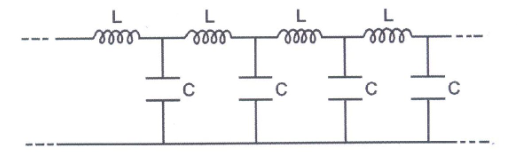
\includegraphics[scale = 0.75]{Figures/monolatticeanalog.png}
        \caption{Electrical analogue of linear mono-atomic lattice}
        \label{fig:monoanalog}
    \end{figure}
    The dispersion relation for this circuit is
    \begin{equation}
        \omega^2 = \dfrac{2}{LC}(1-\cos \theta)
    \end{equation}
    where $\theta$ the phase change introduced by each section (unit cell) of the filter. Thus, one has a precise analogy with the one dimensional mono-atomic lattice, with $C \leftrightarrow m$ and $(1/L) \leftrightarrow f$. From here, it is possible to measure the phase difference between the input and output voltages of the circuit shown in figure (\ref{fig:monoanalog}) as a function of frequency, and from the dispersion relation can be verified.
    \par
    The di-atomic lattice with alternative masses $m$ and $M$ shown in figure (\ref{fig:dilattice}) can be simulated by the transmission line with alternative capacitors $C$ and $C_1$, shown in figure (\ref{fig:dianalog}). The dispersion relations for the mechanical and electrical analogues are given below:
    \begin{equation}
        \omega_{\pm}^2 = f \Bigg(\dfrac{1}{m} + \dfrac{1}{M}\Bigg) + f \Bigg[ \Bigg(\dfrac{1}{m} + \dfrac{1}{M}\Bigg)^2 - \dfrac{4 \sin^2 \theta}{mM} \Bigg]^{1/2}
    \end{equation}
    (mechanical)
    \begin{equation}
        \omega_{\pm}^2 = \dfrac{1}{L} \Bigg(\dfrac{1}{C} + \dfrac{1}{C_1}\Bigg) + \dfrac{1}{L} \Bigg[ \Bigg(\dfrac{1}{C} + \dfrac{1}{C_1}\Bigg)^2 - \dfrac{4 \sin^2 \theta}{CC_1} \Bigg]^{1/2}
    \end{equation}
    (electrical).
    \begin{figure}
        \centering
        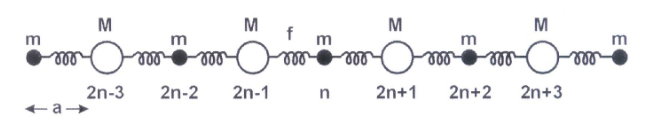
\includegraphics[scale = 0.6]{Figures/diatomiclattice.png}
        \caption{Linear diatomic lattice of lattice parameter $a$ mass $m$ and $M$ and force constant $f$}
        \label{fig:dilattice}
    \end{figure}
    \begin{figure}
        \centering
        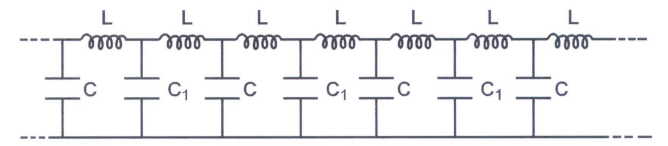
\includegraphics[scale = 0.6]{Figures/diatomiclatticeanalog.png}
        \caption{Electrical analogue of linear di-atomic lattice}
        \label{fig:dianalog}
    \end{figure}
    In contrast to the mono-atomic lattice, there are now two frequencies $\omega_{+}$ and $\omega_{-}$ (corresponding to a particular value of the wave vector $k$. In a plot of $\nu$ versus $\theta$ this leads to two branches; the one corresponding to $\nu_{-}$ is called the acoustical branch and the one corresponding to $\nu_{+}$ is called the optical branch. The frequency gap between the two branches depends on ($M/m$).
    \par
    Thus the diatomic lattice vibration has two cut off frequencies called the acoustic and optical branches. The frequencies, acoustical and optical branches at the energy gap are,
    \begin{equation}
        \begin{split}
            \nu_{+} &= \dfrac{1}{\pi} \sqrt{\dfrac{1}{LC}} \\
            \nu_{-} &= \dfrac{1}{\pi} \sqrt{\dfrac{1}{LC_1}}
        \end{split}
    \end{equation}
    Wavelike solutions do not exist for frequencies between the two cut off frequencies. This is the characteristic energy gap.
    \begin{figure}
        \centering
        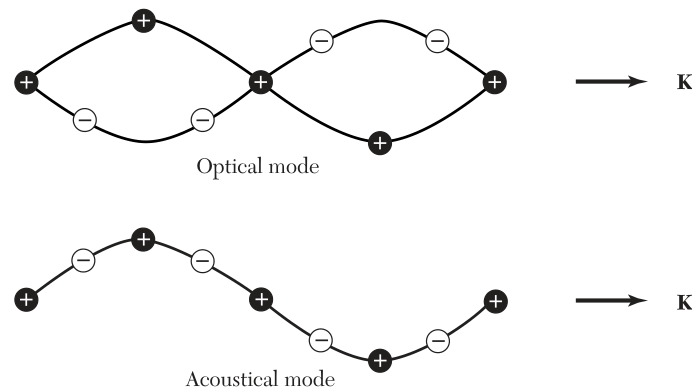
\includegraphics[scale = 0.55]{Figures/optical_acoustic.png}
        \caption{Acoustic and Optical branch}
        \label{fig:modesbranch}
    \end{figure}
    \subsection{Phonons}
    A phonon is a collective excitation in a periodic, elastic arrangement of atoms or molecules in condensed matter, specifically in solids and some liquids. Often referred to as a quasiparticle, it is an excited state in the quantum mechanical quantization of the modes of vibrations for elastic structures of interacting particles. Phonons can be thought of as quantized sound waves, similar to photons as quantized light waves.
    \begin{figure}
        \centering
        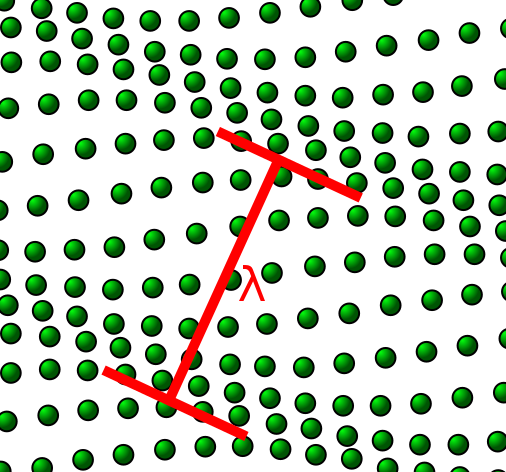
\includegraphics[scale = 0.40]{Figures/506px-Lattice_wave.svg.png}
        \caption{Phonon propagating through a square lattice (atom displacements greatly exaggerated)}
        \label{fig:phonon}
    \end{figure}
    \par
    In order to solve the many-body problem of lattice dynamics two important approximations are usually imposed. First, the sum is only performed over neighboring atoms. Although the electric forces in real solids extend to infinity, this approximation is still valid because the fields produced by distant atoms are effectively screened. Secondly, the potentials $V$ are treated as \textit{harmonic} potentials. This is permissible as long as the atoms remain close to their equilibrium positions. Formally, this is accomplished by Taylor expanding $V$ about its equilibrium value to quadratic order, giving $V$ proportional to the displacement $x^2$ and the elastic force simply proportional to $x$. The error in ignoring higher order terms remains small if $x$ remains close to the equilibrium position.
    \par
    The resulting lattice may be visualized as a system of balls connected by springs. The following figure shows a cubic lattice, which is a good model for many types of crystalline solid. Thus we arrive at our model of Bravais latices we started with.
        \subsubsection{Lattice Waves}
        Due to the connections between atoms, the displacement of one or more atoms from their equilibrium positions gives rise to a set of vibration waves propagating through the lattice. One such wave is shown in the figure (\ref{fig:phonon}). The amplitude of the wave is given by the displacements of the atoms from their equilibrium positions. The wavelength $\lambda$ is marked.
        \par
        Not every possible lattice vibration has a well-defined wavelength and frequency. However, the normal modes do possess well-defined wavelengths and frequencies.
        \subsubsection{Dispersion relation}
        The connection between frequency and wavevector, $\omega = \omega(k)$, is known as a dispersion relation (equation (\ref{eq:branch})). From the results obtained in previous section, in the two roots of $\omega$, the plus sign results in the so-called optical mode, and the minus sign to the acoustic mode. In the optical mode two adjacent different atoms move against each other, while in the acoustic mode they move together.
        \begin{figure}
            \centering
            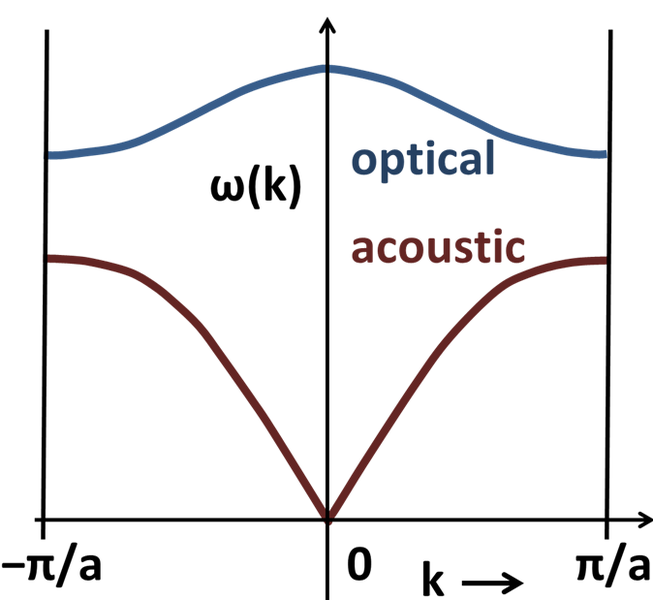
\includegraphics[scale = 0.4]{Figures/653px-Diatomic_phonons.png}
            \caption{Dispersion curves in linear diatomic chain}
            \label{fig:dispersion}
        \end{figure}
        \begin{figure}
            \centering
            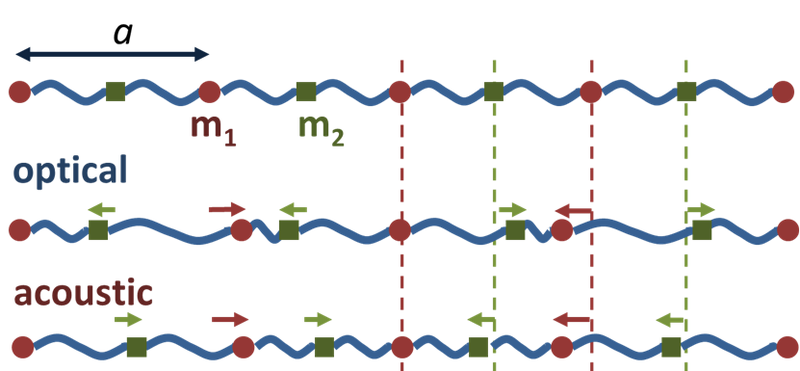
\includegraphics[scale = 0.4]{Figures/800px-Optical_&_acoustic_vibrations.png}
            \caption{Optical and acoustic vibrations in a linear diatomic chain}
            \label{fig:op/ac}
        \end{figure}
\section{Observations}
    The following preliminary observations were made:
    \begin{enumerate}
        \item Average inductance of the inductors used, $L = \SI{1.059}{\milli \henry}$
        \item  Average capacitance of the capacitors used, $C = \SI{52.95}{\nano \farad}$ and $C_1 = \SI{165.52}{\nano \farad}$.
    \end{enumerate}
    \par
    The observation made for monoatomic lattice composed of five cells is tabulated in (\ref{tab:5mono}) and plotted with theoretical values in figure (\ref{fig:5mono}). The corresponding data is tabulated with ten cells is tabulated in (\ref{tab:10mono}) and plotted in figure (\ref{fig:10mono}). Similarly the observations made for diatomic lattice composed of four cells is tabulated in (\ref{tab:4di}) and plotted in figure (\ref{fig:4di}). The amplitude variation with frequency for diatomic lattice was also observed and is tabulated in table (\ref{tab:amplitude}) and plotted in figure (\ref{fig:amplitude}).
    \par
    From here, the theoretical value of the frequency for monoatomic lattice can be found as
    \begin{equation}
        \nu = \dfrac{1}{\pi} \sqrt{\dfrac{1}{LC}} = \SI{47.44}{\kilo \hertz}
    \end{equation}
    From tables (\ref{tab:5mono}) and (\ref{tab:10mono}), the observed cut-off frequency using the fit parameter was found to be around  $\SI{46.45}{\kilo \hertz}$.
    \begin{table*}[]
    \caption{Readings of phase difference for the monoatomic lattice with frequency in an electrical analogue circuit composed of five LC oscillators}
    \label{tab:5mono}
    \setlength{\tabcolsep}{23pt}
    \begin{tabular}{@{}cccc@{}}
    \toprule
    \begin{tabular}[c]{@{}c@{}}\textbf{Phase difference}\\ (deg)\end{tabular} & \begin{tabular}[c]{@{}c@{}}\textbf{Phase difference} \textbf{per unit cell}\\ (deg)\end{tabular} & \begin{tabular}[c]{@{}c@{}}\textbf{Observed frequency}\\ ($\si{\kilo \hertz}$)\end{tabular} & \begin{tabular}[c]{@{}c@{}}\textbf{Theoretical frequency}\\ ($\si{\kilo \hertz}$)\end{tabular} \\ \midrule
    45 & 9 & 0.3 & 3.3 \\
    90 & 18 & 7.5 & 6.6 \\
    135 & 27 & 15 & 9.9 \\
    180 & 36 & 22.3 & 13.1 \\
    225 & 45 & 30 & 16.3 \\
    270 & 54 & 34.9 & 19.3 \\
    315 & 63 & 40.4 & 22.2 \\
    360 & 72 & 43.4 & 25.0 \\ \bottomrule
    \end{tabular}
    \end{table*}
    \begin{figure}
        \centering
        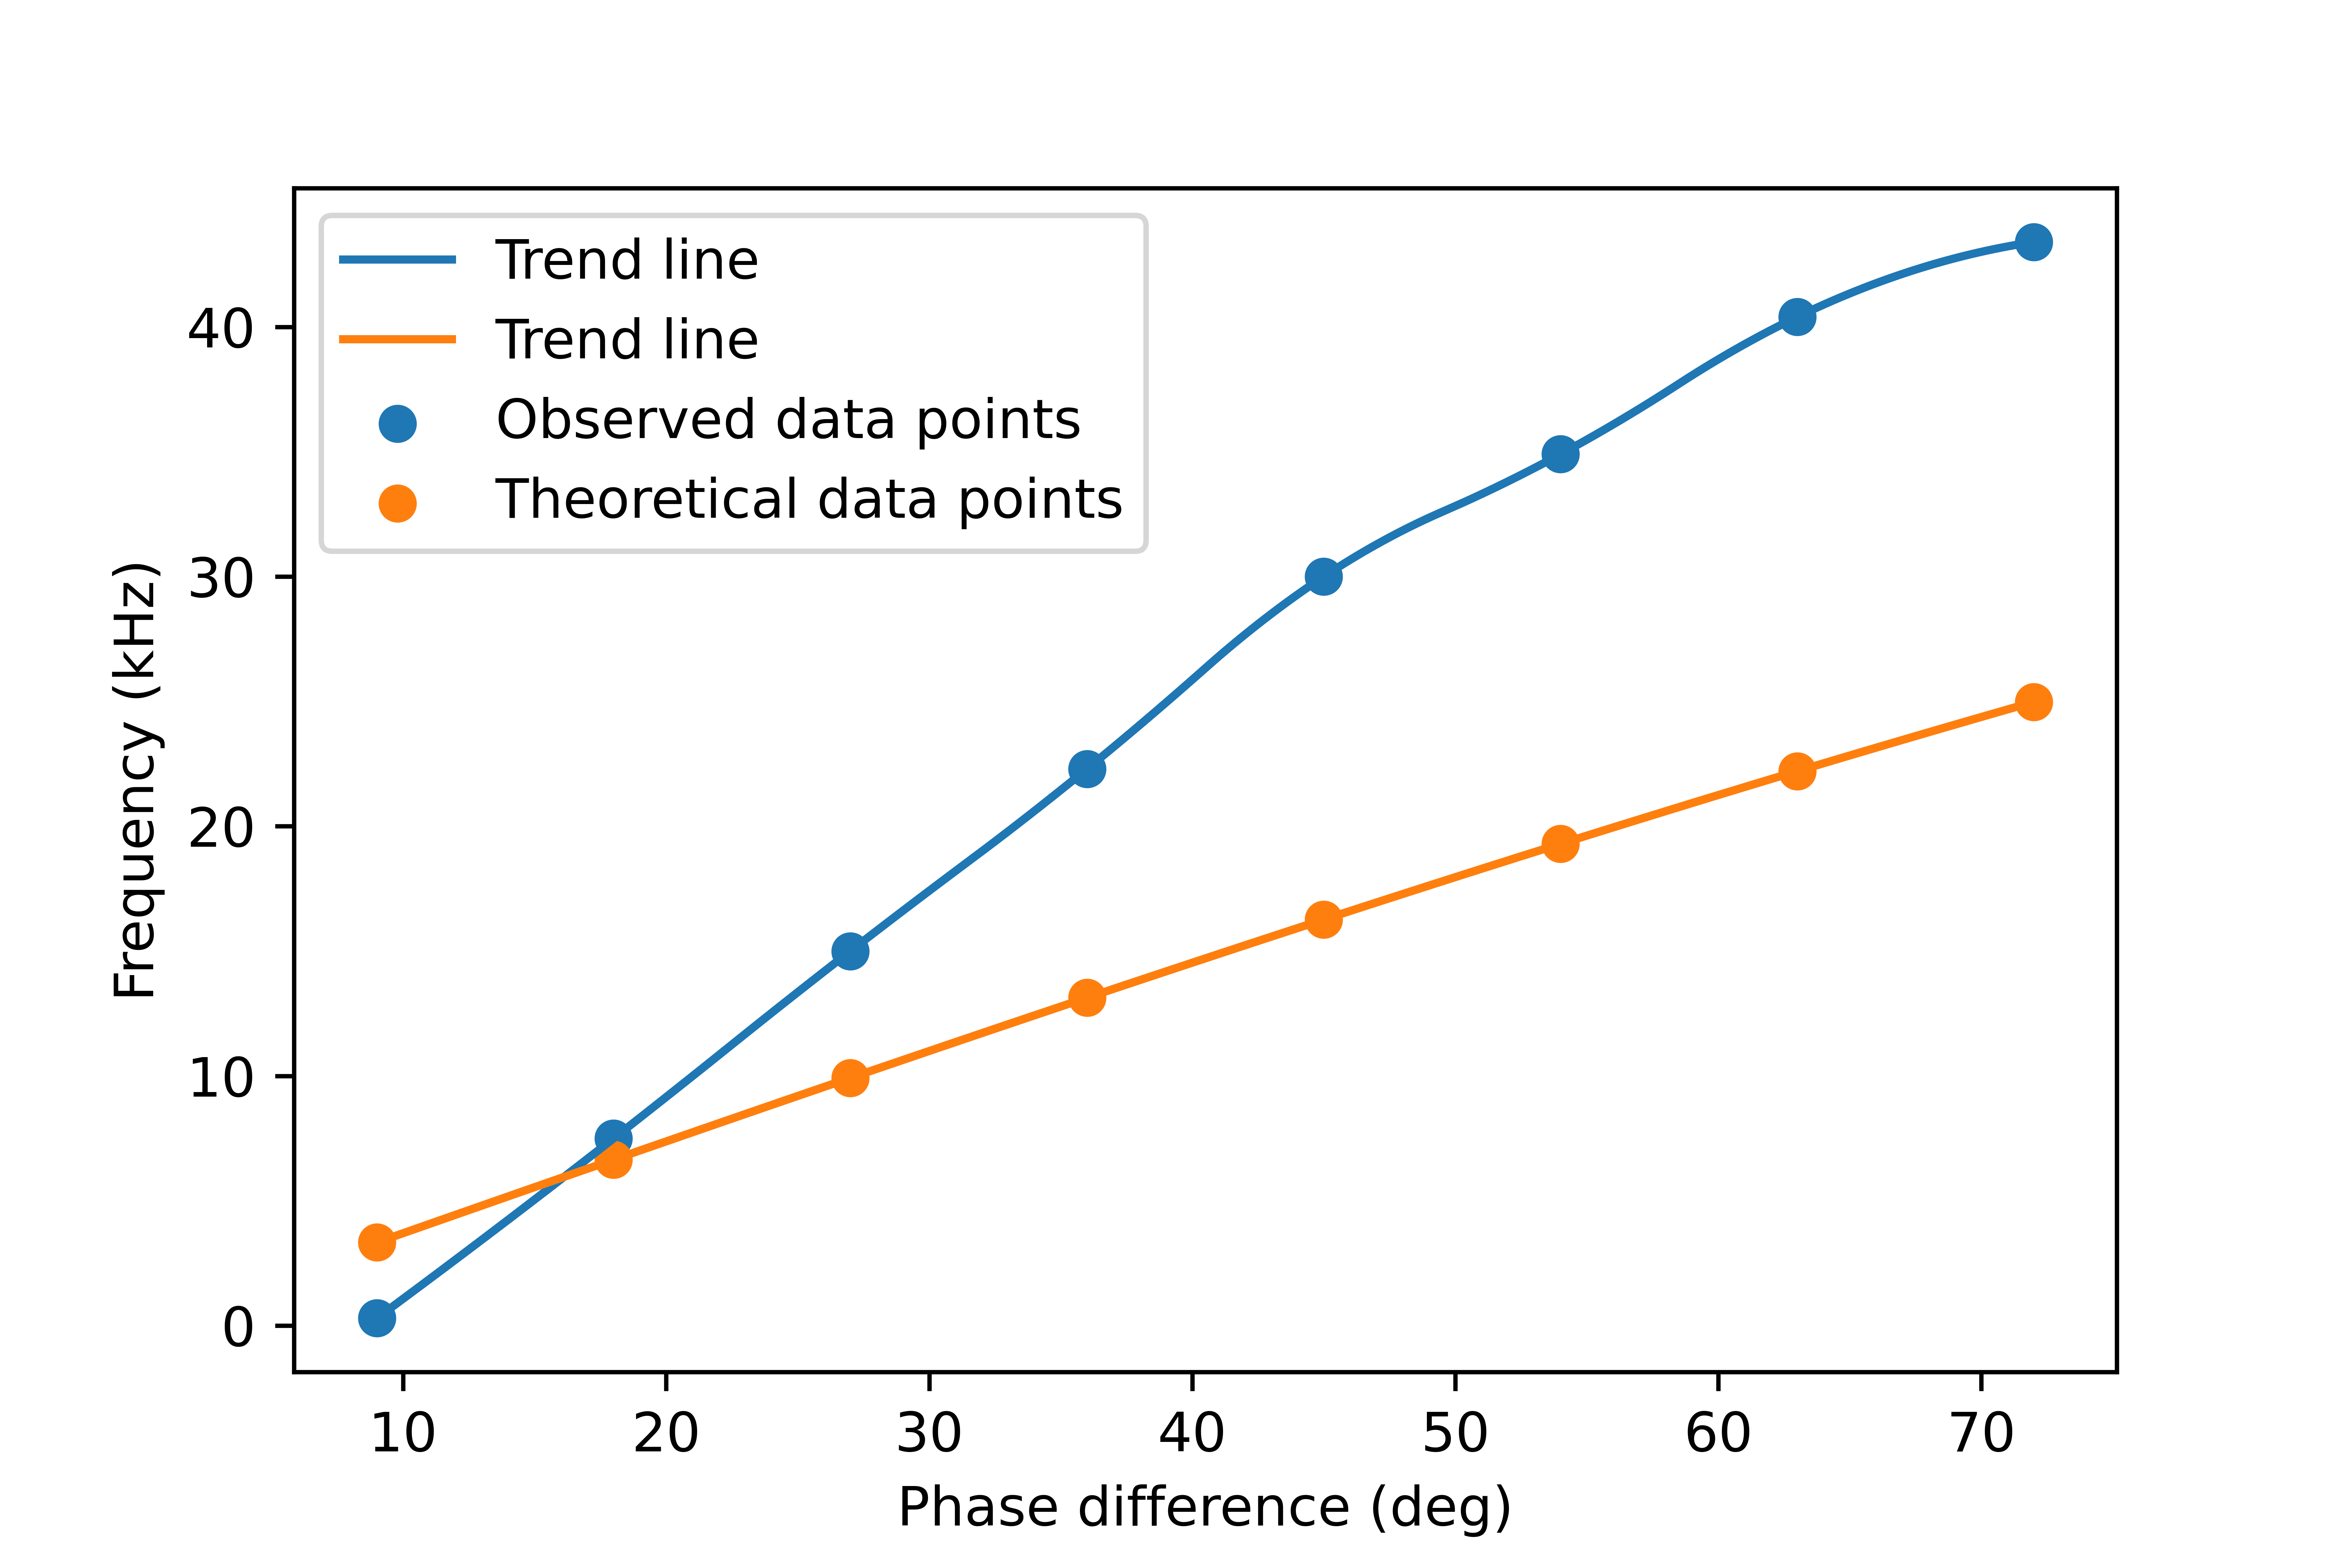
\includegraphics[scale = 0.56]{Figures/plot-mono.png}
        \caption{Plot of frequency versus phase difference for the monoatomic lattice with frequency in an electrical analogue circuit composed of five LC oscillators}
        \label{fig:5mono}
    \end{figure}
    
    \begin{table*}[]
    \caption{Readings of phase difference for the monoatomic lattice with frequency in an electrical analogue circuit composed of ten LC oscillators}
    \label{tab:10mono}
    \setlength{\tabcolsep}{23pt}
    \begin{tabular}{@{}cccc@{}}
    \toprule
    \begin{tabular}[c]{@{}c@{}}\textbf{Phase difference}\\ (deg)\end{tabular} & \begin{tabular}[c]{@{}c@{}}\textbf{Phase difference} \textbf{per unit cell}\\ (deg)\end{tabular} & \begin{tabular}[c]{@{}c@{}}\textbf{Observed frequency}\\ ($\si{\kilo \hertz}$)\end{tabular} & \begin{tabular}[c]{@{}c@{}}\textbf{Theoretical frequency}\\ ($\si{\kilo \hertz}$)\end{tabular} \\ \midrule
    45 & 4.5 & 0.1 & 1.7 \\
    90 & 9 & 3.6 & 3.3 \\
    135 & 13.5 & 7.5 & 5.0 \\
    180 & 18 & 11 & 6.6 \\
    225 & 22.5 & 15 & 8.3 \\
    270 & 27 & 18.6 & 9.9 \\
    315 & 31.5 & 22.3 & 11.5 \\
    360 & 36 & 25.3 & 13.1 \\
    405 & 40.5 & 28.8 & 14.7 \\
    450 & 45 & 31.3 & 16.3 \\
    495 & 49.5 & 34.6 & 17.8 \\
    540 & 54 & 37.1 & 19.3 \\
    585 & 58.5 & 39.2 & 20.8 \\
    630 & 63 & 41 & 22.2 \\
    675 & 67.5 & 43.1 & 23.6 \\
    720 & 72 & 44.7 & 25.0 \\
    765 & 76.5 & 46.4 & 26.3 \\ \bottomrule
    \end{tabular}
    \end{table*}
    \begin{figure}
        \centering
        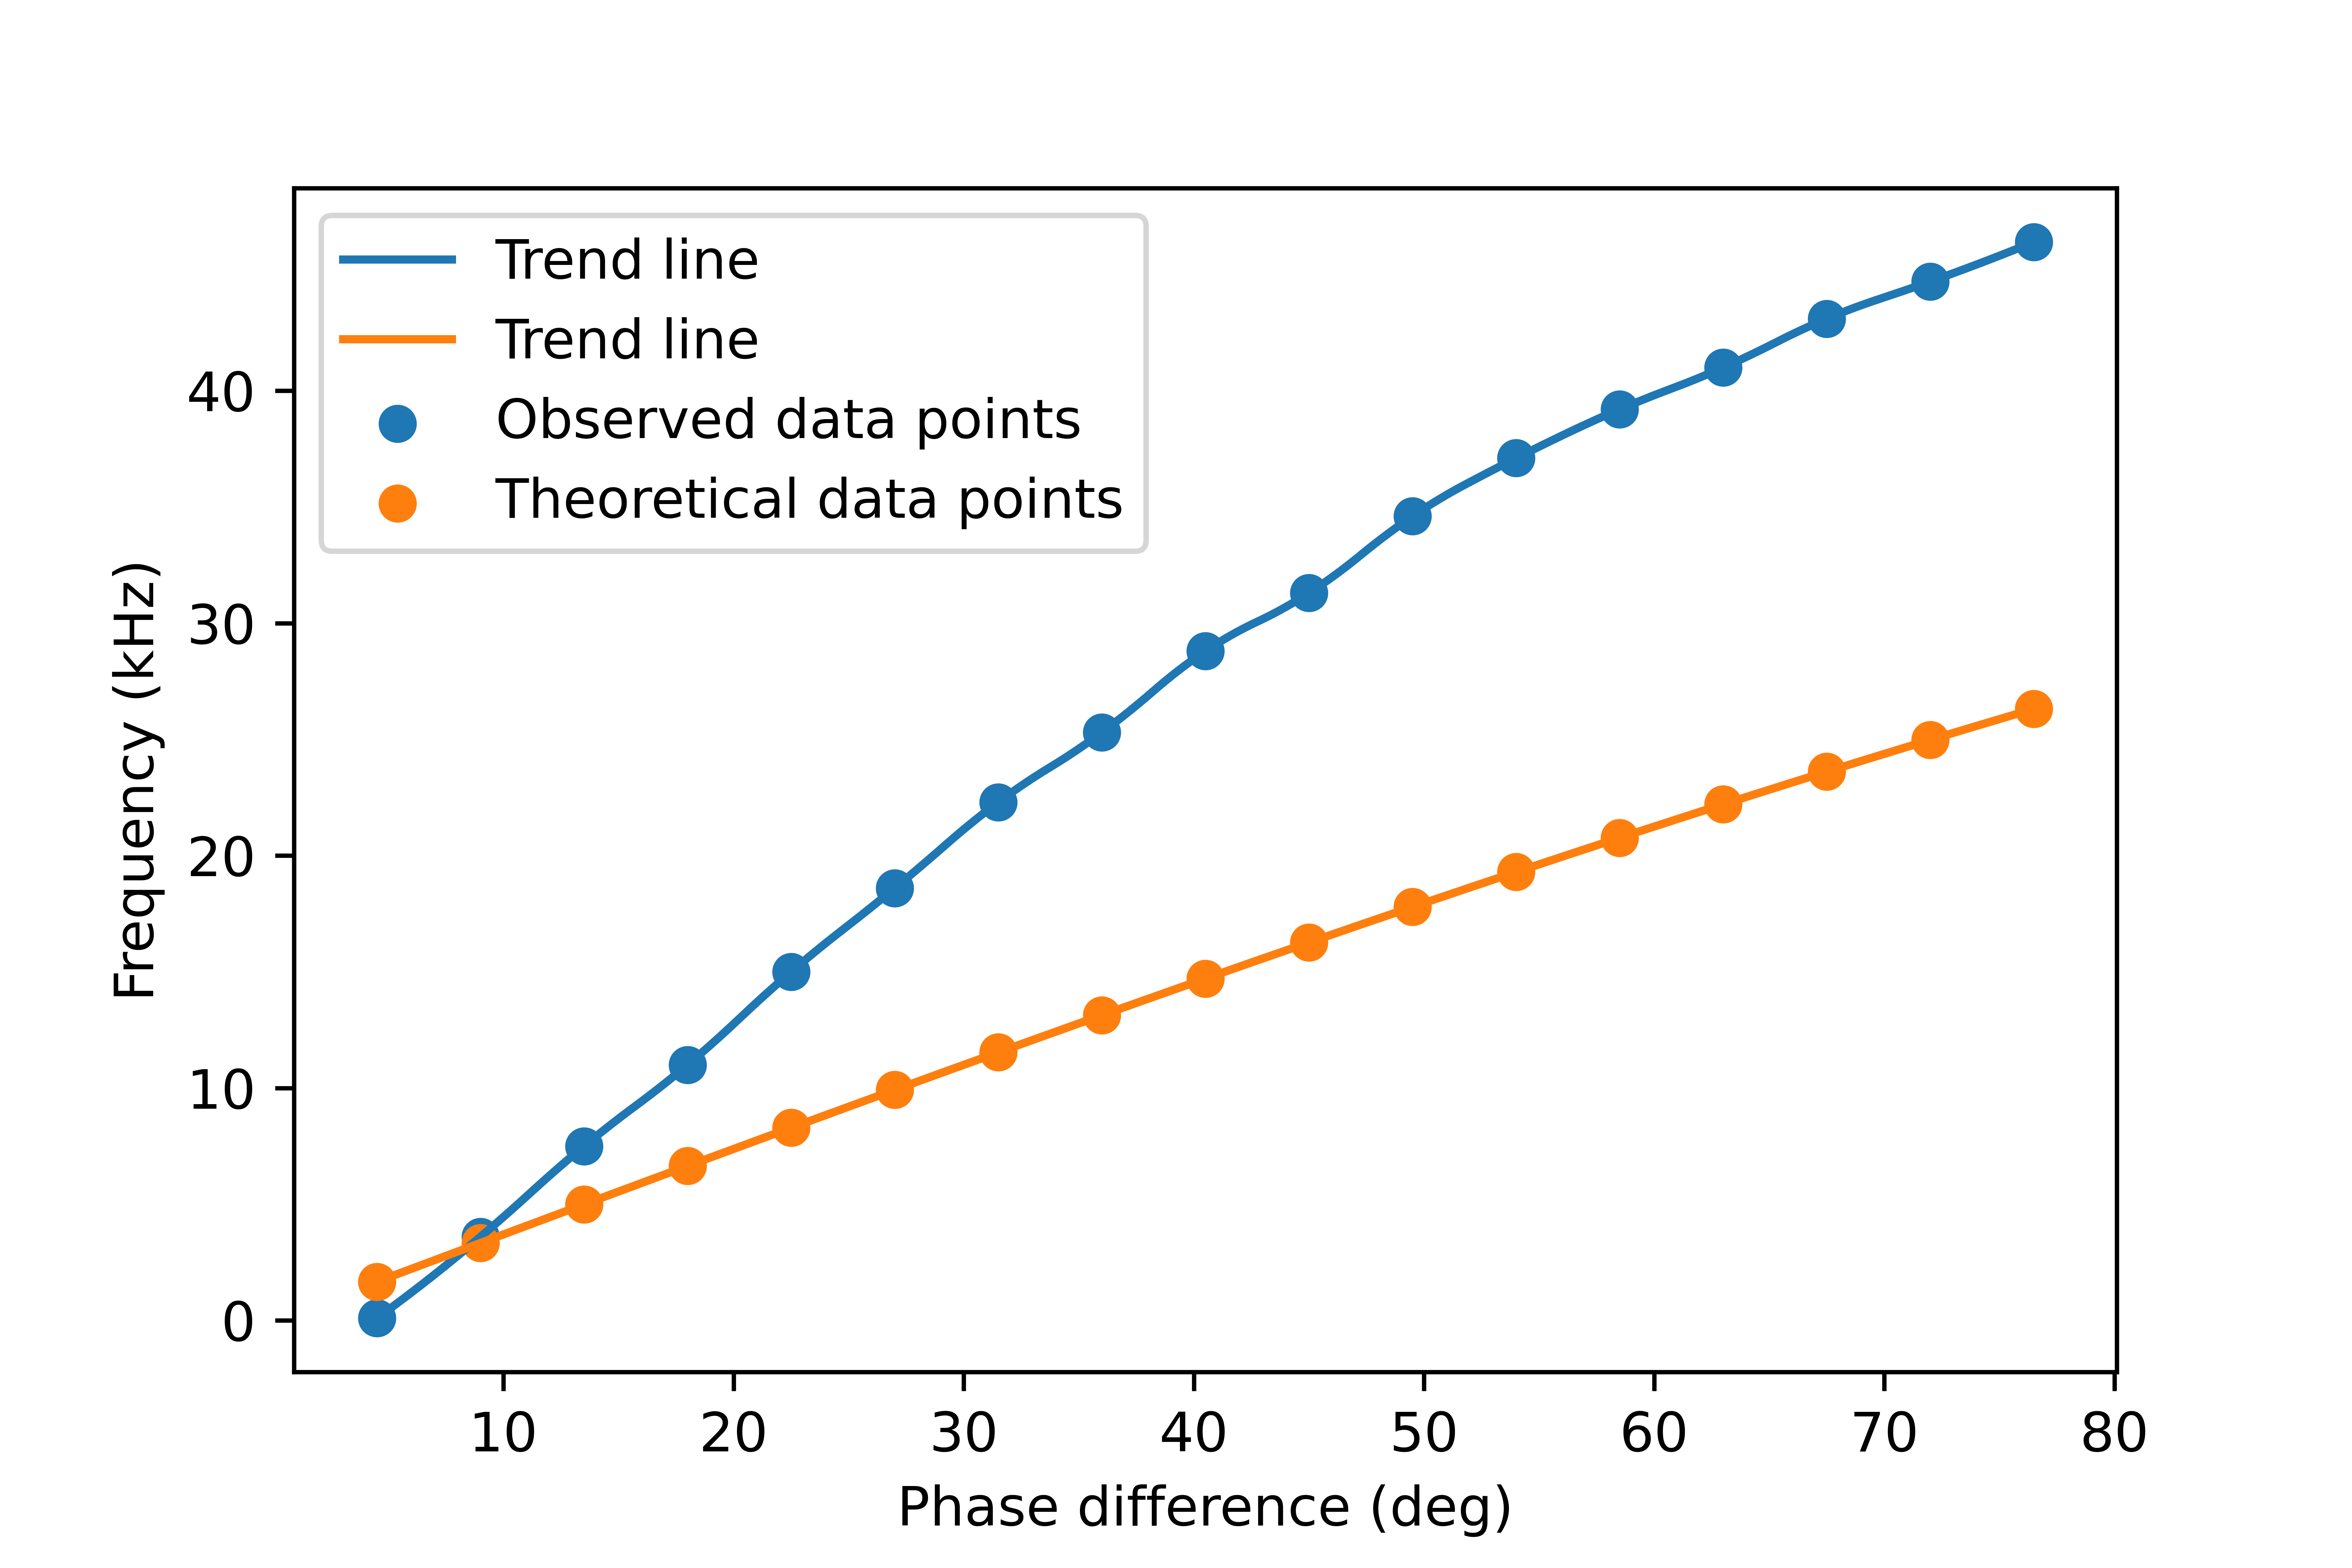
\includegraphics[scale = 0.56]{Figures/plot-di.png}
        \caption{Plot of frequency versus phase difference for the monoatomic lattice with frequency in an electrical analogue circuit composed of ten LC oscillators. The fit parameter $a = \SI[separate-uncertainty=true]{41.234 \pm 1.043}{\kilo \radian \per \second}$}
        \label{fig:10mono}
    \end{figure}

    \begin{table}[]
    \caption{Readings of phase difference for the diatomic lattice with frequency in an electrical analogue circuit composed of four LC oscillators}
    \label{tab:4di}
    \begin{tabular}{@{}ccc@{}}
    \toprule
    \begin{tabular}[c]{@{}c@{}}\textbf{Phase difference}\\ (deg)\end{tabular} & \begin{tabular}[c]{@{}c@{}}\textbf{Phase difference}\\ \textbf{per unit cell}\\ (deg)\end{tabular} & \begin{tabular}[c]{@{}c@{}}\textbf{Observed frequency}\\ ($\si{\kilo \hertz}$)\end{tabular} \\ \midrule
    45 & 11.25 & 0.1 \\
    90 & 22.5 & 2.4 \\
    135 & 33.75 & 5.2 \\
    180 & 45 & 7.8 \\
    225 & 56.25 & 10.4 \\
    270 & 67.5 & 12.7 \\
    315 & 78.75 & 15.3 \\
    360 & 90 & 17.5 \\
    405 & 101.25 & 23.4 \\
    450 & 112.5 & 26.9 \\
    495 & 123.75 & 29.5 \\
    540 & 135 & 31.7 \\
    585 & 146.25 & 33.4 \\
    630 & 157.5 & 34.9 \\
    675 & 168.75 & 36.5 \\
    720 & 180 & 37.9 \\ \bottomrule
    \end{tabular}
    \end{table}
    \begin{figure}
        \centering
        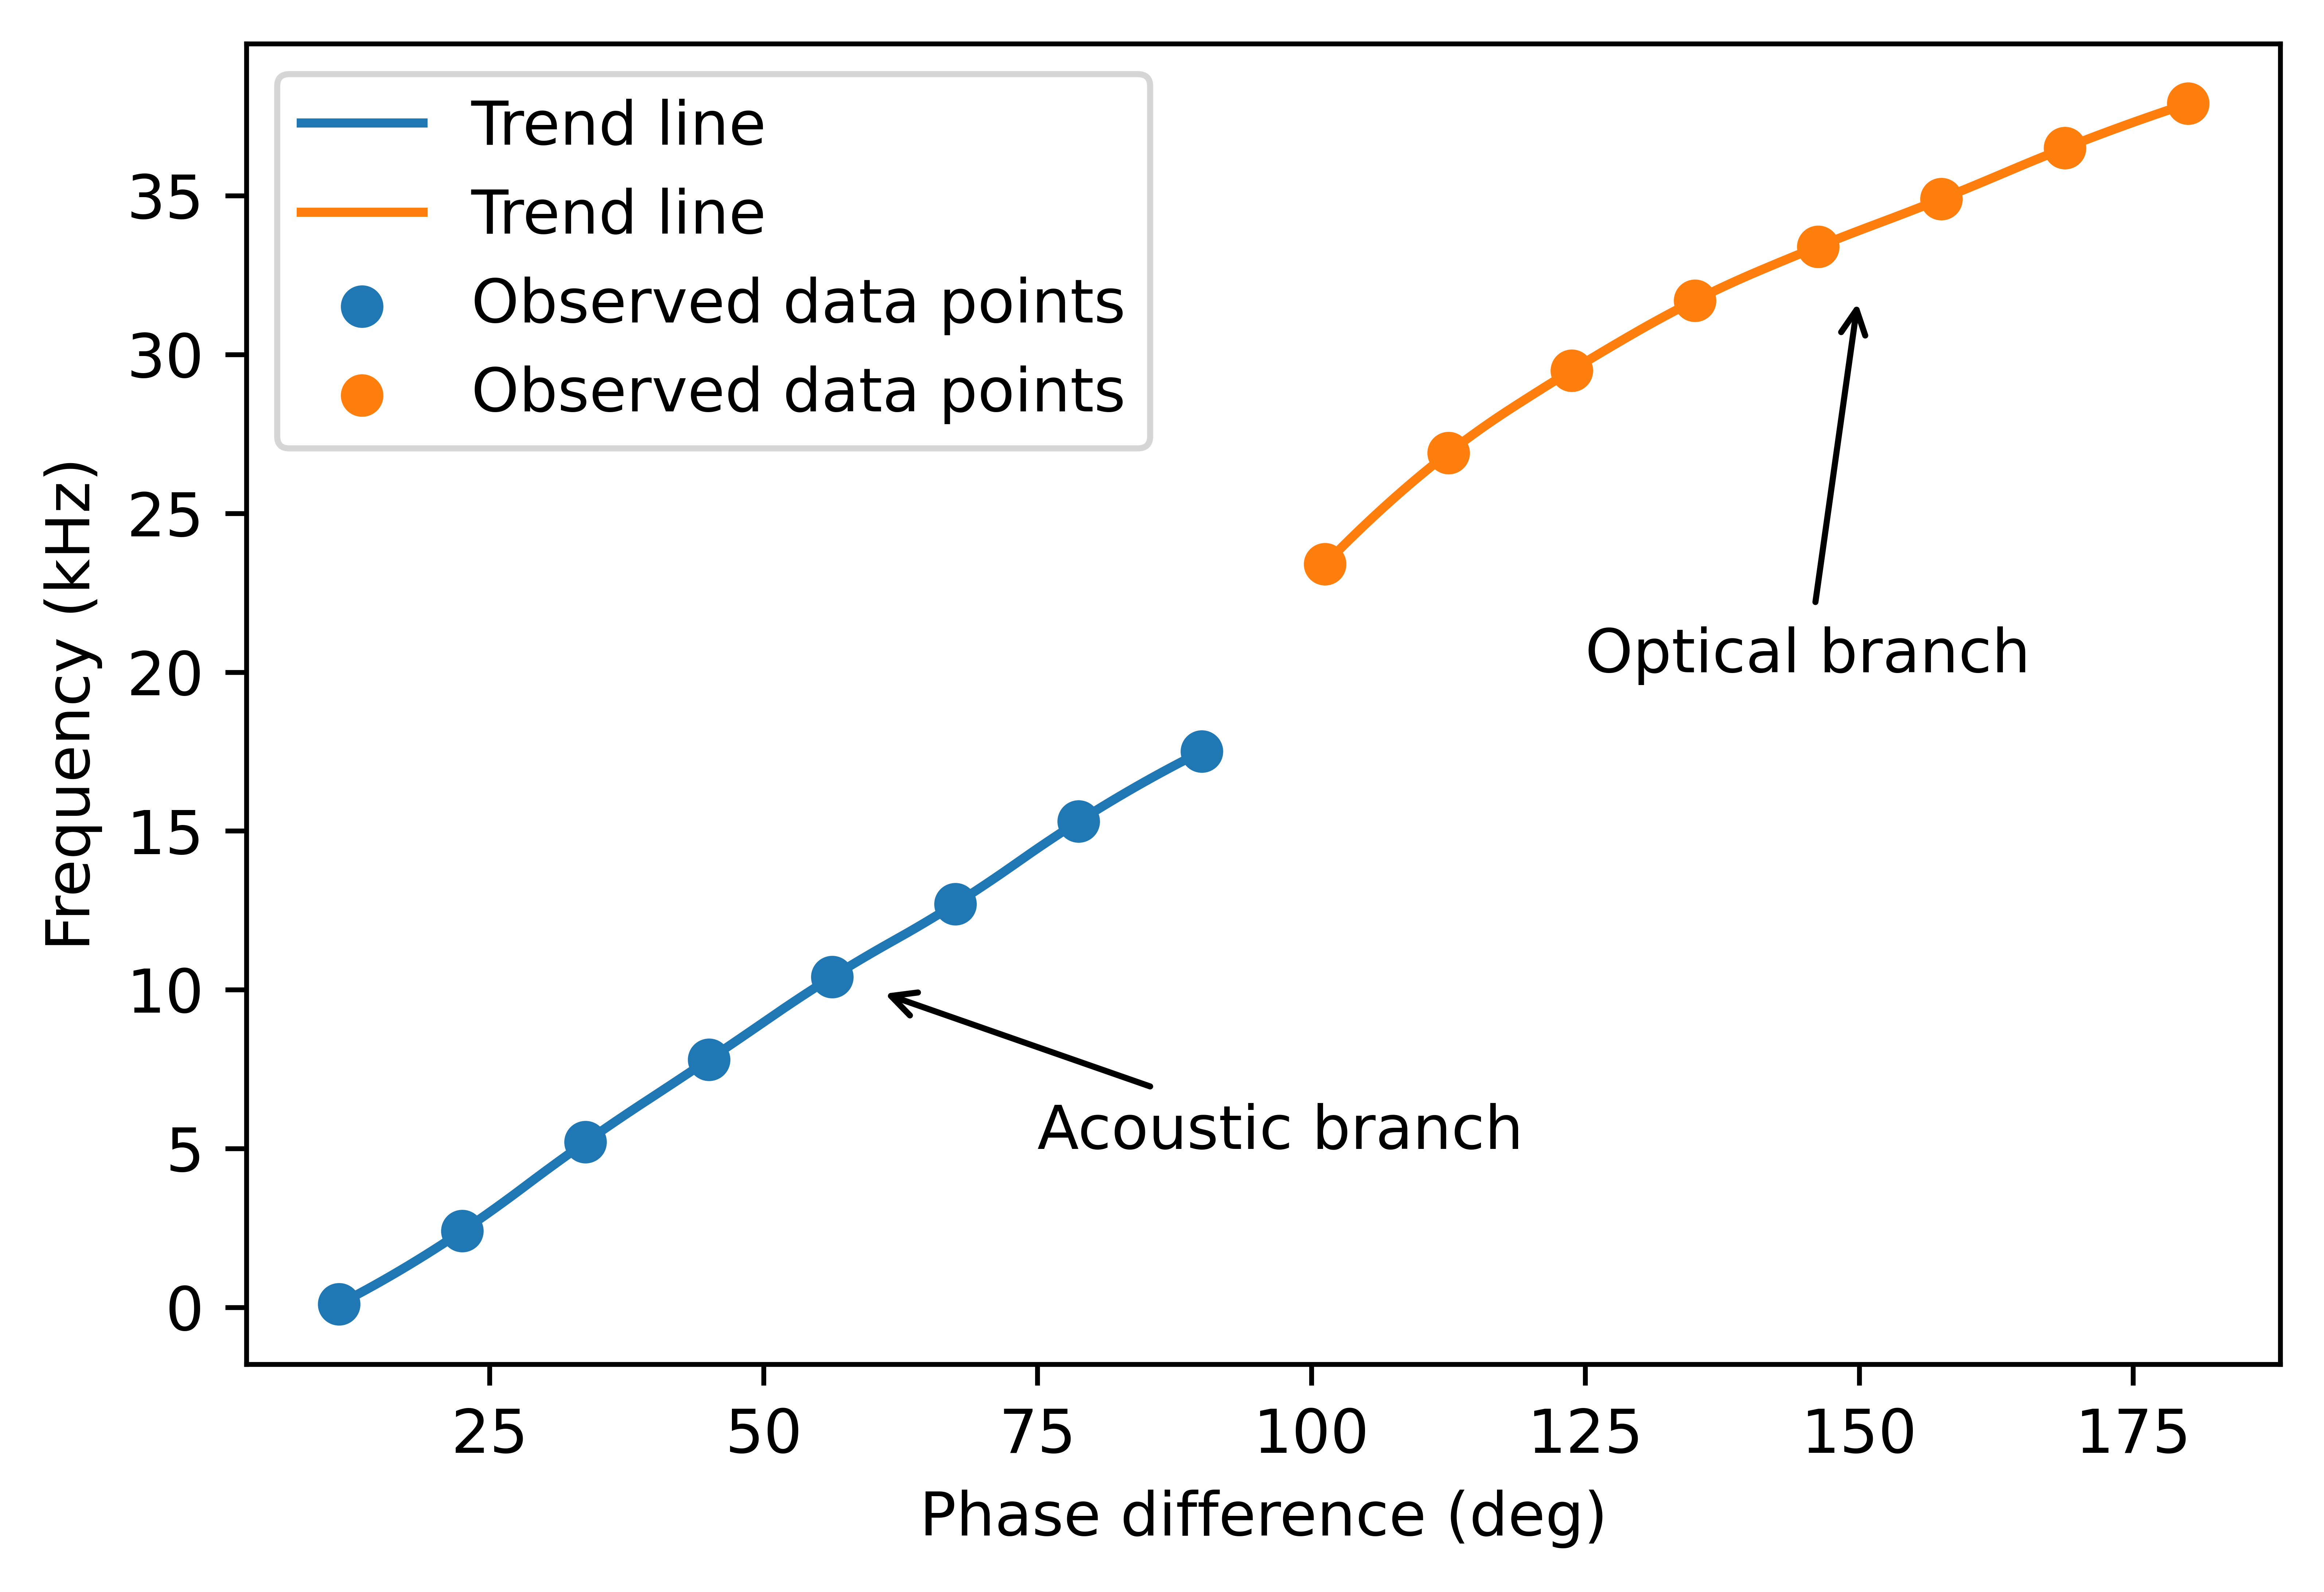
\includegraphics[scale = 0.56]{Figures/plot-bandgap.png}
        \caption{Plot of frequency versus phase difference for the diatomic lattice with frequency in an electrical analogue circuit composed of four LC oscillators. The band gap is clearly visible.}
        \label{fig:4di}
    \end{figure}
    \par
    For the diatomic lattice, the theoretical cut-off frequencies are
    \begin{equation}
        \begin{split}
            \nu_{+} &= \dfrac{1}{\pi} \sqrt{\dfrac{1}{LC}} = \SI{42.51}{\kilo \hertz} \\
            \nu_{-} &= \dfrac{1}{\pi} \sqrt{\dfrac{1}{LC_1}} = \SI{24.04}{\kilo \hertz}
        \end{split}
    \end{equation}
    From tables (\ref{tab:4di}) and (\ref{tab:amplitude}), the observed cut-off frequency was found to be around $\nu_{-} = \SI{23.4}{\kilo \hertz}$ and $\nu_{+} = \SI{39}{\kilo \hertz}$. Therefore the observed band gap value was found to be $\SI{5.9}{\kilo \hertz}$.
    \begin{table}[]
    \caption{Readings of amplitude for the diatomic lattice with frequency in an electrical analogue circuit composed of four LC oscillators}
    \label{tab:amplitude}
    \setlength{\tabcolsep}{12pt}
    \begin{tabular}{@{}cccc@{}}
    \toprule
    \begin{tabular}[c]{@{}c@{}}\textbf{Frequency} \\ ($\si{\kilo \hertz}$)\end{tabular} & \begin{tabular}[c]{@{}c@{}}\textbf{Amplitude} \\ ($\si{\milli \volt}$)\end{tabular} & \begin{tabular}[c]{@{}c@{}}\textbf{Frequency} \\ ($\si{\kilo \hertz}$)\end{tabular} & \begin{tabular}[c]{@{}c@{}}\textbf{Amplitude} \\ ($\si{\milli \volt}$)\end{tabular} \\ \midrule
    1 & 392 & 22 & 12.8 \\
    2 & 356 & 23 & 12.4 \\
    3 & 292 & 23.5 & 12.8 \\
    4 & 244 & 24 & 12.8 \\
    5 & 228 & 24.5 & 13.8 \\
    6 & 232 & 25 & 15.2 \\
    7 & 254 & 25.5 & 17.2 \\
    8 & 242 & 26 & 19.6 \\
    9 & 210 & 27 & 23.4 \\
    10 & 188 & 28 & 19.6 \\
    11 & 188 & 29 & 15.8 \\
    12 & 188 & 30 & 14.4 \\
    13 & 160 & 31 & 14.2 \\
    14 & 126 & 32 & 14.2 \\
    15 & 108 & 33 & 14.6 \\
    16 & 96 & 34 & 14.6 \\
    17 & 78 & 35 & 12.8 \\
    18 & 50.4 & 36 & 9.8 \\
    19 & 31.2 & 37 & 6.4 \\
    20 & 21.6 & 38 & 3.4 \\
    21 & 16 & 39 & 1.4 \\ \bottomrule
    \end{tabular}
    \end{table}
    \begin{figure}
        \centering
        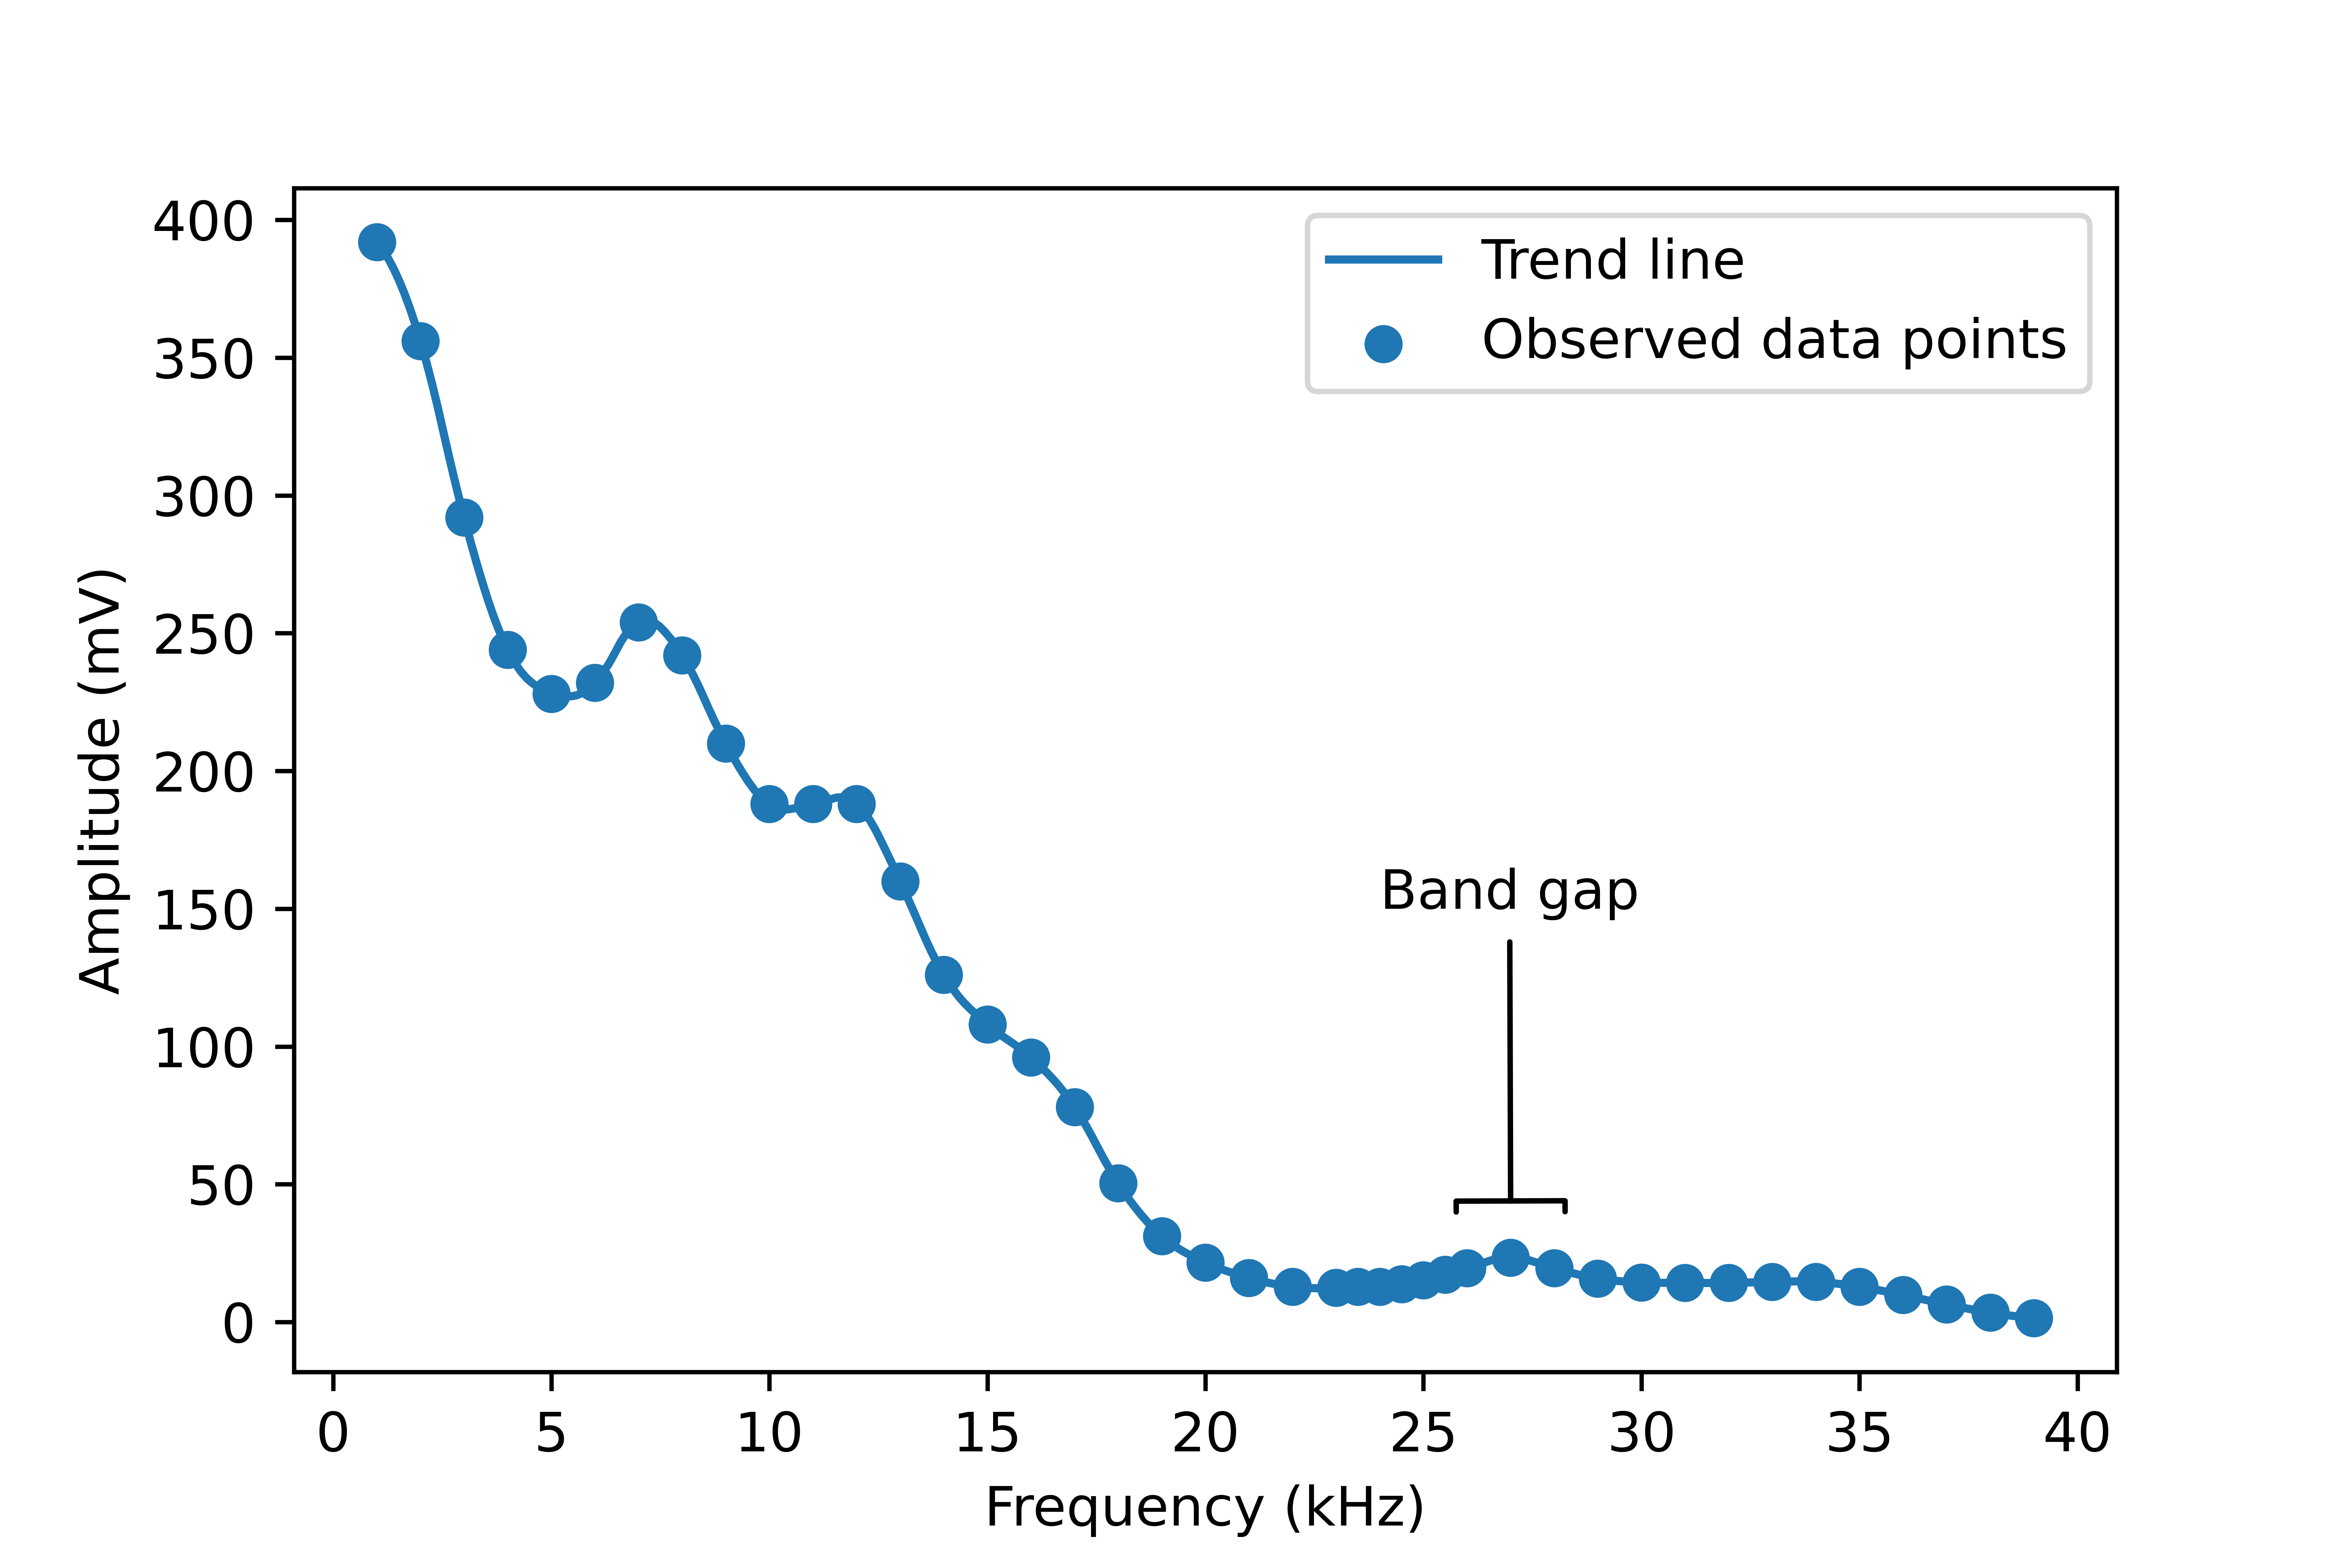
\includegraphics[scale = 0.56]{Figures/plot-amplitude.png}
        \caption{Plot of amplitude versus frequency for the diatomic lattice with frequency in an electrical analogue circuit composed of four LC oscillators. The band gap region has been marked.}
        \label{fig:amplitude}
    \end{figure}
\section{Error Analysis}
    Relative error in cut-off frequency for the cut-off frequency
    \begin{equation}
        \begin{split}
            \delta &= \dfrac{\nu_{exp} - \nu_{th}}{\nu_{th}} \times 100\% \\
            &= \dfrac{46.45-47.44}{46.45} \\
            &= -2.13 \%
        \end{split}
    \end{equation}
    \par
    Absolute error in cut-off frequency can be calculated using the fitting parameter $\delta a = \SI{1.04}{\kilo \hertz}$.
    \begin{equation}
        \delta \nu_{max} = \nu_{max} \sqrt{\Big(\dfrac{\delta a}{a}\Big)^2} = \SI{1.17}{\kilo \hertz}
    \end{equation}
    or direct from the formula
    \begin{equation}
        \delta \nu_{max} = \nu_{max} \sqrt{\Big(\dfrac{\delta L}{L}\Big)^2+\Big(\dfrac{\delta C}{C}\Big)^2} = \SI{1.71}{\kilo \hertz}
    \end{equation}
    \par
    We can proceed likewise for the diatomic lattice and absolute error in thw two cut-off frequencies are
    \begin{equation}
        \begin{split}
            \delta \nu_{+} &= \nu_{+} \sqrt{\Big(\dfrac{\delta L}{L}\Big)^2+\Big(\dfrac{\delta C}{C}\Big)^2} = \SI{1.13}{\kilo \hertz} \\
            \delta \nu_{-} &= \nu_{-} \sqrt{\Big(\dfrac{\delta L}{L}\Big)^2+\Big(\dfrac{\delta C_1}{C_1}\Big)^2} = \SI{1.21}{\kilo \hertz}
        \end{split}
    \end{equation}
    
\section{Results}
    \begin{enumerate}
        \item Experimental cutoff frequency for monoatomic lattice vibrations was found to be $\nu = \SI[separate-uncertainty=true]{46.45\pm 1.17}{\kilo \hertz}$
        \item The acoustical cut-off frequency for diatomic lattice vibrations was found to be $\nu_{-} = \SI[separate-uncertainty=true]{24.04\pm 1.21}{\kilo \hertz}$.
        \item The optical cut-off frequency for diatomic lattice vibrations was found to be $\nu_{-} = \SI[separate-uncertainty=true]{42.51\pm 1.13}{\kilo \hertz}$.
    \end{enumerate}

\section{Discussions}
    \begin{enumerate}
        \item A phonon is the quantum mechanical description of an elementary vibrational motion in which a lattice of atoms or molecules uniformly oscillates at a single frequency.
        \item In classical mechanics this designates a normal mode of vibration. Normal modes are important because any arbitrary lattice vibration can be considered to be a superposition of these elementary vibration modes (cf. Fourier analysis). While normal modes are wave-like phenomena in classical mechanics, phonons have particle-like properties too, in a way related to the wave–particle duality of quantum mechanics.
        \item Compared to the static lattice model that deals with the average positions of atoms in a crystal; lattice dynamics works towards extending the concept of crystal lattice to an array of atoms with finite masses capable of motion. The motion of masses is a superposition of vibrations of atoms around the equilibrium sites induced by the interaction with neighboring atoms. The collective vibration of the atoms within the crystal forms a wave of allowed wavelength and amplitude. For example, as we know that light is said to be a wave motion composed of photons, we can also think of the normal modes of vibration in a solid as being a particle. One major problem with Lattice dynamics is that is hard to find the normal modes of vibration of the crystal.
        \item In a 3-D crystal, the atoms vibrate in three dimensions with three vibrational branches, one longitudinal and two transverse. For a 3-D Lattice with N atom per lattice point, there is $3(m-1)$ optical branches, of which $2(m-1)$ are transverse optical phonons and the remaining phonons are longitudinal optical phonons. In a transverse wave, the atomic displacement direction is perpendicular to the direction of the propagated wave. The remaining two transverse waves will overlap if the two vibrational directions are symmetric. In regards to electrons, the phonons are dispersed along different crystallographic direction.
        \item Phonons are to sound waves in a solid what photons are to light: they are the quanta that carry it. The dispersion relation of phonons is also non-trivial and important, being directly related to the acoustic and thermal properties of a material. For most systems, the phonons can be categorized into two main types: those whose bands become zero at the center of the Brillouin zone are called acoustic phonons, since they correspond to classical sound in the limit of long wavelengths. The others are optical phonons, since they can be excited by electromagnetic radiation. 
        \item Inelastic neutron scattering is an experimental technique commonly used in condensed matter research to study atomic and molecular motion as well as magnetic and crystal field excitations. Here, the neutron exchanges energy with the atoms in a material and when a neutron is scattered by a crystalline solid, it can absorb or emit an amount of energy equal to a quantum of phonon energy, . This gives rise to inelastic coherent scattering in which the neutron energy before and after the scattering differ by an amount, $h \nu$ (i.e. \textit{energy transfer}).
    \end{enumerate}

\section{Conclusions}
    \begin{enumerate}
        \item From the value of percentage relative error, it is evident that the experimental value of the cutoff frequency of mono-atomic lattice matches with an high degree of accuracy with the predicted theoretical value.
        \item The fit did not converge for the diatomic lattice vibrations even after 4000 iterations. So, the fitting was done using the same fit equation for monoatomic lattice as shown in the graph. However, the existence of energy gap is evident from the plot.
        \item This experiment helped in the understanding of the dynamics of lattice vibrations via an electrical simulation of the same. The fact that Lattice vibrations can be can be modelled as an oscillator is exploited and the lattice is considered to be made of an infinite spring mass system.
        \item From the results, for the monoatomic lattice, a very good match between the experimental and theoretical values can be seen.
        \item In the case of diatomic lattice, the theoretical and experimental values are close but further comments cannot be made due to the non convergence of fitting.
    \end{enumerate}
    
\section{Precautions}
    \begin{enumerate}
        \item Make sure all the components are connected properly.
        \item Do not disturd the setup while taking the measurements.
    \end{enumerate}

\end{document}
%
% ****** End of file aipsamp.tex ******